%% uctest.tex 11/3/94
%% Copyright (C) 1988-2004 Daniel Gildea, BBF, Ethan Munson.
%
% This work may be distributed and/or modified under the
% conditions of the LaTeX Project Public License, either version 1.3
% of this license or (at your option) any later version.
% The latest version of this license is in
%   http://www.latex-project.org/lppl.txt
% and version 1.3 or later is part of all distributions of LaTeX
% version 2003/12/01 or later.
%
% This work has the LPPL maintenance status "maintained".
% 
% The Current Maintainer of this work is Daniel Gildea.

\documentclass[11pt]{ucthesis}

%% The graphicx package provides the includegraphics command.
\usepackage{graphicx}
\graphicspath{{../../../latex/graphics/}{./figures/}{./graphics/}}
%% The amssymb package provides various useful mathematical symbols
\usepackage{amssymb}
\usepackage{amsmath}
\usepackage{amsthm}
\usepackage{mathtools}
\usepackage{braket}
\usepackage{enumerate, enumitem}


\def\dsp{\def\baselinestretch{2.0}\large\normalsize}
\dsp
\begin{document}

% Declarations for Front Matter

\title{FASTPas - Fast Predictive Ariel Scanning}
\author{Sargis S Yonan}
\degreeyear{2018}
\degreemonth{June}
\degree{MASTER OF SCIENCE}
\chair{Professor Gabriel Hugh Elkaim}
\committeememberone{Professor Numero Dos}
\committeemembertwo{Professor Numero Tres}
\numberofmembers{3} %% (including chair) possible: 3, 4, 5, 6
\deanlineone{Dean Tyrus Miller}
\deanlinetwo{Vice Provost and Dean of Graduate Studies}
\deanlinethree{}
\field{COMPUTER ENGINEERING}
\emphasis{ROBOTICS AND CONTROL}
\campus{Santa Cruz}

\begin{frontmatter}

\maketitle
\copyrightpage

\tableofcontents
\listoffigures
\listoftables

\begin{abstract}
Unmanned Aerial Vehicles (UAVs) have become more prevalent in fields of work and study that benefit from having a birds eye view on a given situation. Firefighter teams have been using UAVs to find the origin of fires, and where fires are spreading to. Scientific researchers have been using aerial thermal imaging to determine rates of change in ice growth and melting, and thermal exchange between the ocean and atmosphere.
\par
The use of autonomous UAVs could benefit rescue teams, firefighters, scientific re- searchers, and private sector industries in the interest of time and data discovery. Using a single or multiple UAVs in a flying network, an area with fields of interest can be scanned efficiently completely autonomously. By simply drawing on a map the general area wished to be scanned by the autonomous fleet, a deployed pod of these UAVs can stream back, to a ground station, live aerial information. This mapping time can be greatly reduced with the use of statistical interpolation techniques that help the pod or single UAV avoid having to scan an entire region, but rather, have the UAVs scan the areas with the lowest level of confidence in prediction.
\par
The Kriging Method, a popular interpolation tool offers a prediction and a variance of prediction, but is computationally expensive because of constant fitting procedures. We can exploit the Kriging variances generated by our prediction to motivate the UAVs to autonomously steer in the areas of least confidence until a minimum confidence in prediction is achieved for an entire unknown field. By designing a computational efficient algorithm based on a Universal Kriging Method, the system is feasible and could benefit a large group of potential users.
\end{abstract}

\begin{dedication}
\null\vfil
{\large
\begin{center}
To all those who think flying robots are cool, and to my mother, Marina.
\vspace{12pt}
\end{center}}
\vfil\null
\end{dedication}


\begin{acknowledgements}
I want to thank Sharon Rabinovich, who helped me make sense of everything, as well as the rest of the Autonomous Systems Lab at UC Santa Cruz for the support and motivation to continue this project everyday.
\end{acknowledgements}

\end{frontmatter}

\part{Efficient Interpolation}

\chapter{Introduction}
There currently exists no consumer-level UAV system that can autonomously scan a perimeter of area to quickly map an unknown field. Due to the benefits of the solution to the problem, in terms of scientific research and benefit to fire fighting, I believe that designing a modified mathematical statistical interpolation method could make this system possible. Using a modified Kriging Method and a custom autonomous pod-UAV simulation, I would like to demonstrate that the system is possible, and could also benefit a variety of civil servants and scientists. We will, in this chapter, develop the tools and understanding of a method for interpolating data autonomously from just a few measured positions.

\section{Kriging Prediction}
It can be impossible to scan every square unit of area in a field, even with UAVs. Depending on the size of the map, it can often be most beneficial, in the interest of time flying above an area, to get a good enough prediction of the status of a field based off of a limited number of samples.\\
The Universal Kriging Method, also known as the Wiener–Kolmogorov prediction, is a geostatistical Gaussian process historically used to interpolate data in fields varying from natural resource location prediction for mining to real estate value appraisals.\\
Using the Kriging method, the unknown probability of interest at point $s_{0}$ is achieved via:
\begin{equation}
\widetilde{Z}(s_{0})=w_{1}Z(s_{1}) + w_{2}Z(s_{2}) + ... + w_{n}Z(s_{n})
\end{equation}
\begin{center}
	\begin{figure}[h]
		\begin{tabular}{cc}
			\centering
			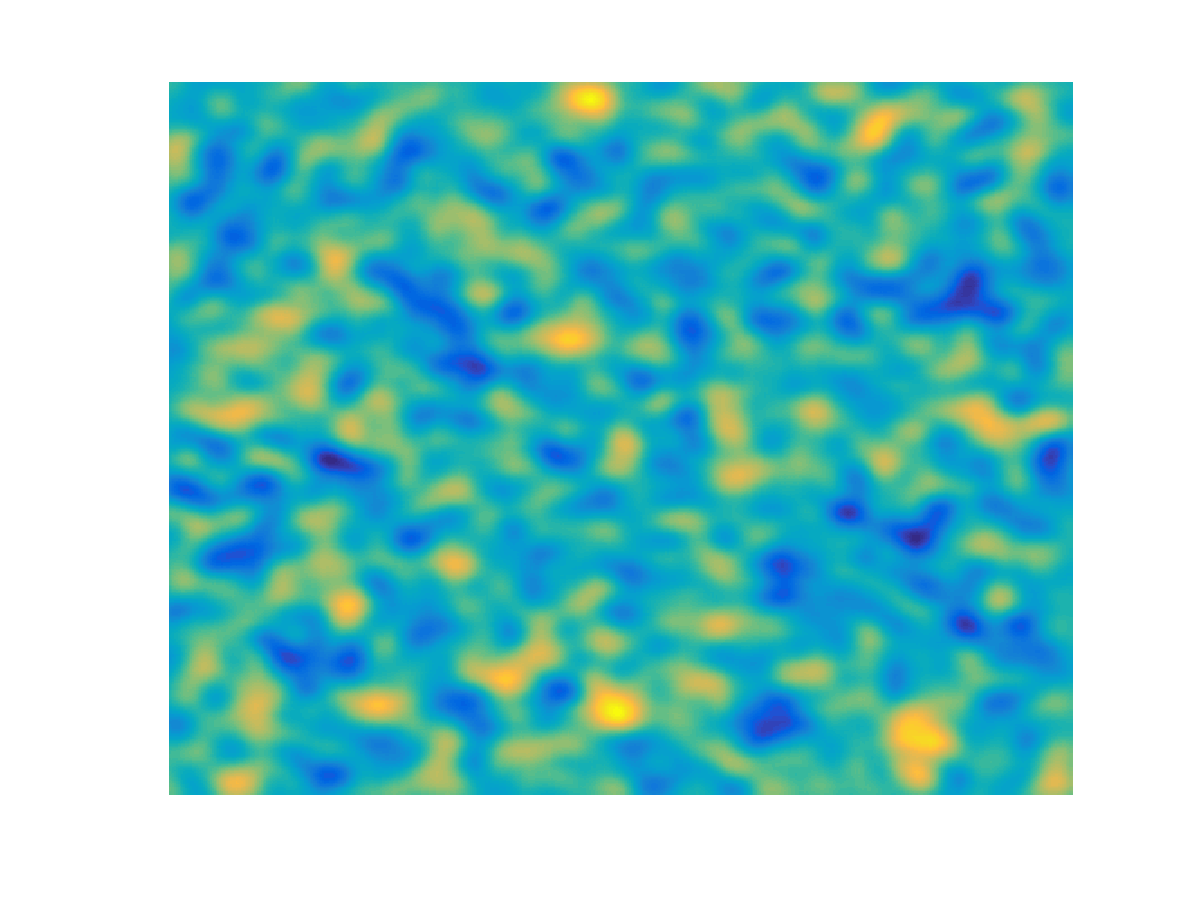
\includegraphics[width=0.49\linewidth]{random_field.eps} &
			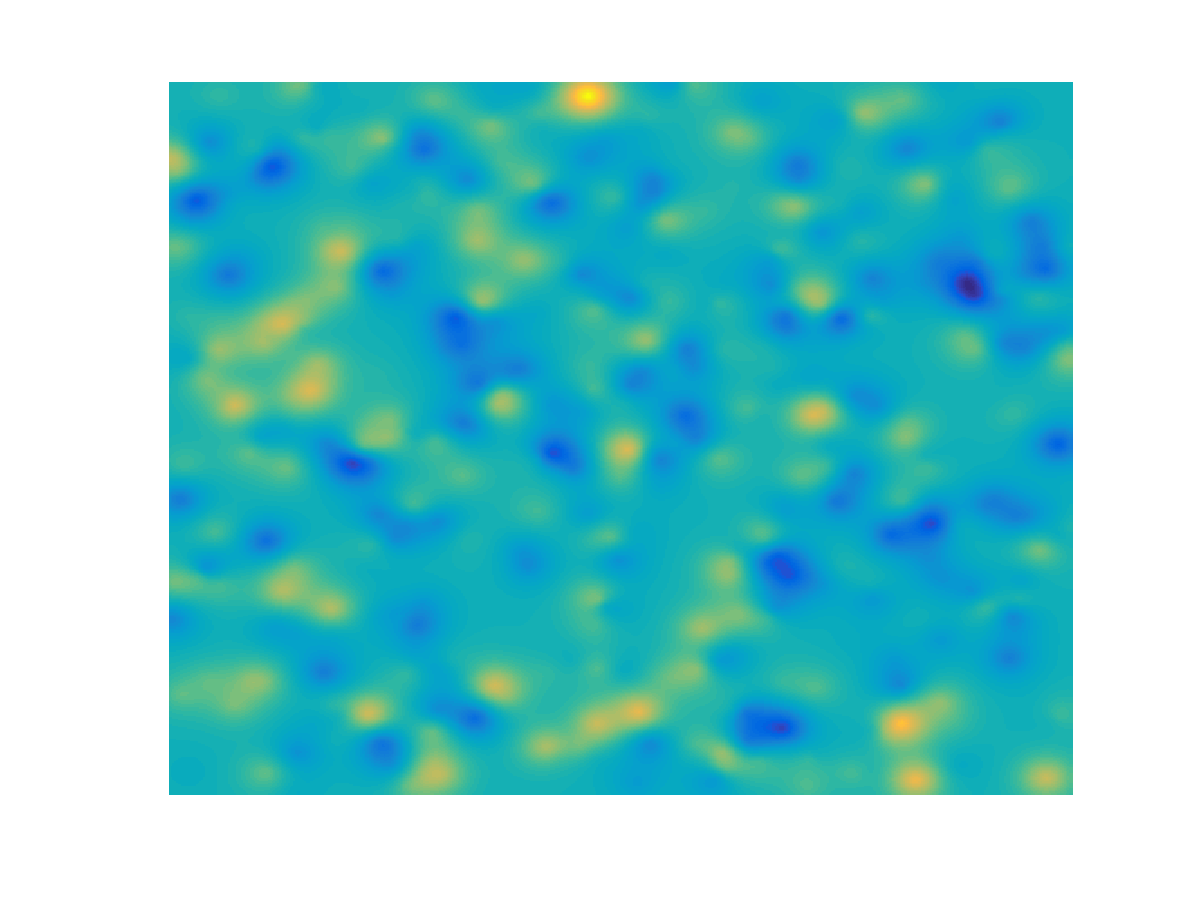
\includegraphics[width=0.49\linewidth]{kriging_prediction.eps} \\
			Randomly Generated Field & Kriging Method Predicted Field\\
		\end{tabular}
		\caption{A comparison of a random field generated using 500 random autocorrelated points, and a prediction of the field using the Kriging Method at randomly sampled points. \textit{figures generated using MATLAB.}}
	\end{figure}
\end{center}
The Kriging method also provides a variogram, with its prediction. The variogram provides a confidence score for each probability it computes via the computation of a discrete semi-variogram:\\
\begin{equation}
\hat{\gamma}({\bf{h}})=\dfrac{1}{2N({\bf{h}})}\sum_{i=1}^{N({\bf{h}})}\Big[Z(s_{i})-Z(s_{i}+{\bf{h}})\Big]^{2}
\end{equation}\\
Where $N({\bf{h}})$ is the number of pairs of data locations that are vector ${\bf{h}}$ apart.\\
The semi-variogram is then fit by a least squares to a continuous variogram that can be sampled for each point at question.
\begin{center}
	\begin{figure}[h]
		\centering
		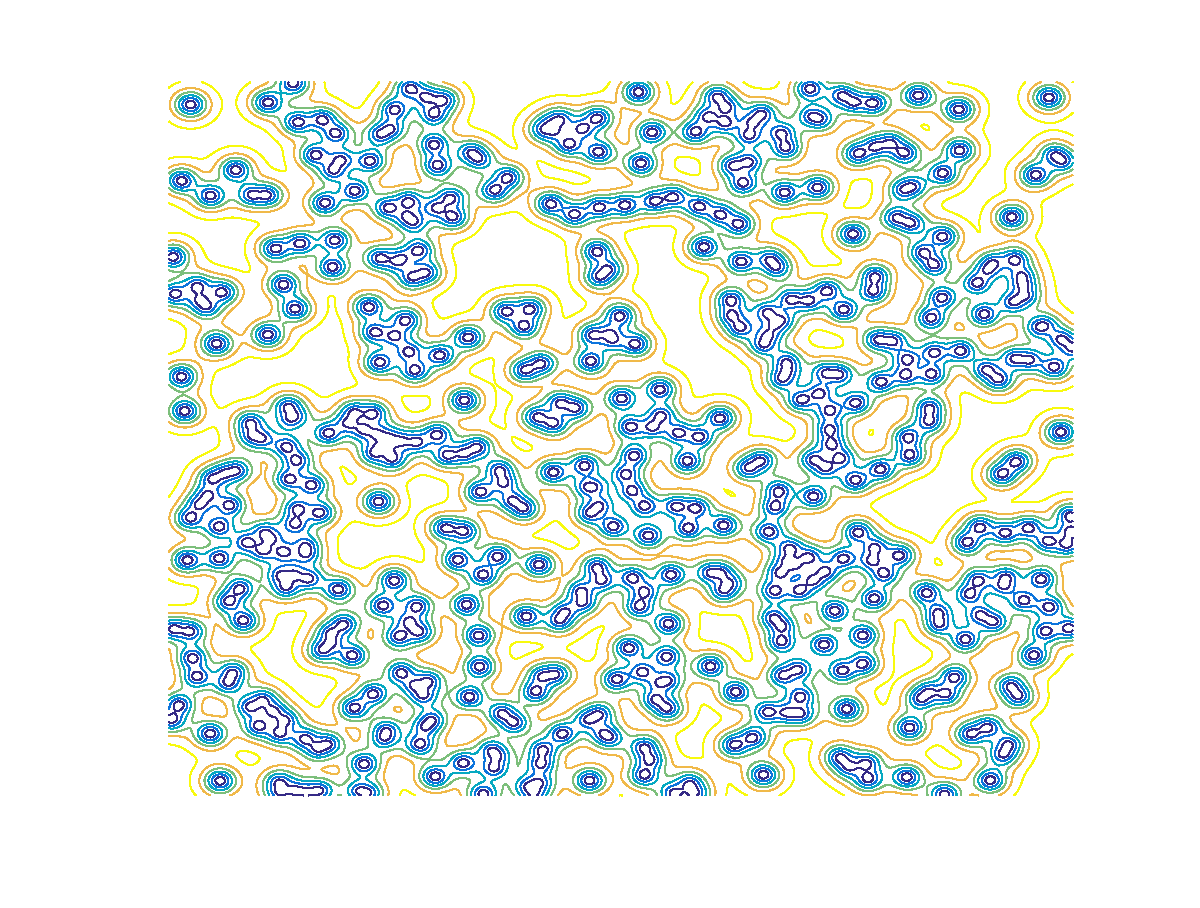
\includegraphics[scale=.5]{kriging_variance.eps}
		\caption{The variance of each prediction point from Figure 1. Larger spacing between the contours indicate greater variance. \textit{figure generated using MATLAB.}}
	\end{figure}
\end{center}
Although the method is optimal for data with no trends or drift, the use of the unmodified Kriging Method technique has the drawback of being computationally intensive and slow to compute in a live and timely manner. This is due to the multiple matrix inversions and least squares fittings to calculate the weights of the interpolation and the continuous variograms. It would be desired, in the case of autonomous UAVs that must constantly steer themselves in the best direction, to quickly calculate probabilities and covariances. \\

\section{Kriging Variance}
\subsection{Semivariogram}
\subsection{Variogram}

\section{Autonmous Waypoint Selection}
\subsection{Searching for low confidence}
\subsection{Selecting points of low confidence}

\section{Natural Neighbor Selection}
\subsection{Voronoi Tesselations}

\chapter{Previous Work}
Some other research was once performed.

\part{Can it fly?}
\chapter{Introduction}

\section{Custom Simulation}
\subsection{Flying Engine}
\subsubsection{Plot Drawing}
\subsubsection{Waypoint Selection}

\section{FastPAS}
\subsection{The Algorithm}
\subsection{Simulating It}

\chapter{Results}

\chapter{Conclusion}
The method has proven to be a powerful interpolation method in simulations for simulated fields. The Kriging method has proven to be a working aerial mapping technique that provides a robust model for predictions and confidence scores. The goal of this thesis will be to design the algorithm for use with a pod of autonomous UAVs. A modified technique will have to first be developed to reduce the computational complexity of the algorithm by autonomously selecting optimal neighborhoods of sub-areas to run the method on.\\
Once the new method has been developed, an accurate simulation demonstrating its effectiveness and potential to be used in a real pod of UAVs will then be created and demonstrated. 
If time and resources are available, the algorithm will be ported to a real pod of UAVs to accomplish the task of autonomous scanning using thermal imaging (via infrared sensors). Tests will be conducted to prove the effectiveness and time efficiency of the newly developed algorithm.

\nocite{*}
\bibliographystyle{plain}
\bibliography{yonan_cmpe_msc_thesis}

\appendix
\chapter{Ancillary Material}
kriging formula
least squares
semi-v to v procedure
calcuylating weights

\end{document}
